% !TEX root = Main.tex
\documentclass[conference]{IEEEtran}

% ======================== PACKAGES ==============================
\usepackage[utf8]{inputenc}
\usepackage[T1]{fontenc}
\usepackage{amsmath,amssymb,amsfonts}
\usepackage{amsthm}
\usepackage{mathtools}
\newtheorem{theorem}{Theorem}
\newtheorem{proposition}{Proposition}
\newtheorem{definition}{Definition}
\newtheorem{remark}{Remark}
\usepackage{bm}
\usepackage{booktabs}
\usepackage{enumitem}
\usepackage{cite}
\usepackage{hyperref}
\usepackage{xcolor}
\usepackage{tikz}
\usetikzlibrary{arrows.meta, positioning, fit, calc}


% ======================== FLOAT SPACING ========================
\setlength{\textfloatsep}{8pt plus 2pt minus 2pt}   % between float and text
\setlength{\floatsep}{6pt plus 2pt minus 2pt}       % between consecutive floats
\setlength{\belowcaptionskip}{-6pt}                  % below caption (inside float)

% ======================== CUSTOM MACROS =========================
% Lie groups and manifolds
\newcommand{\SOthree}{\mathrm{SO}(3)}
\newcommand{\SEthree}{\mathrm{SE}(3)}
\newcommand{\sothree}{\mathfrak{so}(3)}
\newcommand{\Sph}{\mathbb{S}}

% Linear algebra
\newcommand{\R}{\mathbb{R}}
\newcommand{\norm}[1]{\lVert #1 \rVert}
\newcommand{\abs}[1]{\lvert #1 \rvert}
\newcommand{\diag}{\mathrm{diag}}
\newcommand{\tr}{\mathrm{tr}}
\newcommand{\argmin}{\operatornamewithlimits{argmin}}

% Hat and vee maps
\newcommand{\hatmap}[1]{\widehat{#1}}

\renewcommand{\eqref}[1]{Eq. (\ref{#1})}
% ======================== TITLE =================================
\title{Decentralized Geometric Control for Cable-Suspended Payload Transport with Adaptive Mass Estimation}

\author{
  \IEEEauthorblockN{Author Names Omitted for Review}
  \IEEEauthorblockA{Affiliation Omitted for Review}
}

% ================================================================
\begin{document}

\maketitle

% ======================== ABSTRACT ==============================
\begin{abstract}
Cooperative aerial transport---where multiple quadrotors carry a payload via cable suspensions---demands controllers that respect nonlinear manifold geometry, operate without centralized coordination, and enforce safety constraints. We present GPAC, a four-layer hierarchical architecture enabling $N$~quadrotors to transport a cable-suspended payload with \emph{no payload, cable, or adaptive-parameter exchange}. The key insight is \emph{implicit coordination}: each quadrotor independently estimates its payload mass share from local cable measurements, causing the combined forces to converge to the correct total without knowledge of $N$, the payload mass, or any peer's state. Operating directly on the full nonlinear configuration manifold, GPAC integrates geometric position/attitude control with anti-swing regulation, an extended state observer for wind rejection, concurrent learning mass estimation without persistent excitation, and a control barrier function (CBF) safety filter with input-to-state safety guarantees. We prove that CBF-induced force modifications preserve almost-global exponential attitude stability on~$\SOthree$. High-fidelity simulation with flexible cables, onboard sensor fusion, and wind turbulence validates $23.5 \pm 1.5$\,cm payload tracking RMSE at sub-MFLOP per-agent cost.
\end{abstract}

\begin{IEEEkeywords}
Cooperative aerial transport, geometric control, decentralized systems, adaptive estimation, control barrier functions, multi-UAV systems.
\end{IEEEkeywords}

% ======================== SECTIONS ==============================
\section{Introduction}\label{sec:intro}
% !TEX root = ../Main.tex
Cooperative aerial transport uses multiple unmanned aerial vehicles (UAVs) to jointly carry a payload suspended by cables. This increases capacity, workspace, and fault tolerance compared to single platforms. These systems are inherently safety-critical. Cable slack, excessive swing, vehicle tilt, inter-agent collisions, and disturbances can each result in loss of controllability or payload instability. Achieving $N$-quadrotor cooperation requires controllers that respect the nonlinear manifold structure, function without centralized coordination, and systematically address dominant failure modes.

Lee, Sreenath, and Kumar~\cite{lee2010geometric, sreenath2013geometric} formulated cable-suspended transport on the full nonlinear configuration manifold. They achieved almost-global stability without Euler-angle singularities. Later work~\cite{lee2018geometric} added anti-swing regulation of pendular cable dynamics. Sharma and Sundaram~\cite{sharma2023geometric} introduced a geometric controller for multi-UAV payload transfer that does not require link information. Sun et al.~\cite{sun2025agile} demonstrated agile cooperative cable manipulation using online kinodynamic planning. However, these controllers require centralized state knowledge or full-state payload feedback. Each quadrotor must know the number of cooperating agents~$N$ and the payload mass~$m_L$, or all peers' states. This is impractical when communication is unreliable.

Consensus-based formation controllers and distributed optimization approaches use linearized dynamics and Euclidean error metrics. These forfeit global stability during large-angle maneuvers, precisely when guarantees are most critical. Wang et al.~\cite{wang2024automultilift} introduced Auto-Multilift, a distributed learning framework. It tunes model predictive control (MPC) cost functions online for cooperative load transport. However, this approach depends on optimization-based MPC, not geometric control. It does not provide Lyapunov stability certificates. Concurrent learning~\cite{chowdhary2010concurrent, chowdhary2013exponentially} enables convergence without persistent excitation (PE) by utilizing stored data. This is relevant because cooperative hover provides insufficient excitation. Existing concurrent learning applications are restricted to centralized, single-vehicle scenarios.

Cable-suspended transport imposes real-time state constraints. Cables must remain taut, cable angles must be bounded, swing rates must be limited, and collisions must be prevented. Control Barrier Functions (CBFs)~\cite{ames2017control, ames2019control} enforce these constraints via online quadratic programs (QPs) that minimally modify a nominal controller. Yang and Xie~\cite{yang2025robust} combined CBFs with disturbance estimators for single-quadrotor cable-suspended payload safety. They showed that disturbance-observer CBFs reduce conservatism under model uncertainty. However, integrating CBFs with geometric controllers on nonlinear manifolds while preserving Lyapunov certificates remains an open problem. This challenge becomes even more intense in decentralized multi-agent settings, where coupled constraints and attitude stability must be maintained simultaneously.

Most geometric transport studies assume rigid cables and perfect state feedback. In practice, real cables exhibit compliance, wave propagation, and slack-to-taut transitions. These effects significantly influence system behavior~\cite{williams2009dynamics}. Onboard estimation must combine noisy IMU and GPS data using nonlinear filters~\cite{sola2017quaternion}. Wind introduces unmodeled forces. The robustness of geometric cooperative controllers under these conditions remains largely uncharacterized. In summary, no existing framework simultaneously achieves geometric manifold control, decentralized adaptive estimation without persistent excitation, and runtime safety certification for multi-UAV cable transport.

To address these gaps, a central principle in safety-critical engineering is the early identification and systematic mitigation of dominant hazards~\cite{STPAleveson}. Instead of designing a monolithic controller and verifying safety after development, each GPAC layer addresses a specific transport hazard: anti-swing regulation stabilizes pendular modes, adaptive estimation mitigates load uncertainty, the extended state observer (ESO) compensates for disturbances, and the CBF layer enforces constraints as a runtime supervisor. The hierarchical multi-rate structure with timescale separation limits fault propagation, and the fully decentralized implementation eliminates single points of failure~\cite{koopman2017autonomous}. Table~\ref{tab:failure_modes} in Section~\ref{sec:results} validates this mapping with measured data.

Expanding on this principle, the GPAC architecture decomposes the cooperative transport problem into $N$ identical single-agent subproblems based on a key insight: each quadrotor independently estimates its payload mass share $\hat{\theta}_i \approx m_L/N$ from local cable measurements, and the combined forces automatically sum to the correct total:
\begin{equation}
  \sum_{i=1}^{N} F_i = \sum_{i=1}^{N} \hat{\theta}_i \cdot u \;\longrightarrow\; m_L \cdot u,
  \label{eq:force_convergence}
\end{equation}
In this setup, $u := g\,e_3 + \ddot{p}_L^d$ represents the common payload acceleration demand, which is computed identically by every agent from the shared reference. This implicit coordination removes the need for a centralized coordinator, payload or cable state exchange, consensus protocols, or prior knowledge of the payload mass. The specific contributions are as follows:
\begin{enumerate}[leftmargin=*, itemsep=2pt]
  \item The decentralized controller for multi-UAV cable transport operates directly on the nonlinear manifold without linearization, requiring no payload state, cable state, or adaptive-parameter exchange.

  \item Each agent estimates $\hat{\theta}_i \to m_L/N$ from local cable tension and direction with exponential convergence---even during near-hover conditions where classical adaptive laws fail.

  \item A modular safety layer enforcing cable tautness, angle, tilt, swing rate, and collision constraints with input-to-state safety (ISSf) guarantees. Theorem~\ref{thm:compatibility} proves the CBF-induced modifications preserve almost-global exponential attitude stability on $\SOthree$.

  \item High-fidelity Drake-based simulation with bead-chain cables, onboard sensor fusion, and Dryden wind turbulence, achieving $23.5 \pm 1.5$\,cm payload RMSE at sub-MFLOP per-agent cost.
\end{enumerate}


\section{System Modeling}\label{sec:modeling}
% !TEX root = ../Main.tex
The world frame~$\mathcal{W}$ has $e_3$ upward. Rotations lie in $\SOthree$; the hat map $(\cdot)^{\wedge}:\R^3 \to \sothree$ satisfies $\hatmap{v}w = v \times w$. Cable directions $q_i \in \Sph^2$ have tangent projection $P(q) = I_3 - qq^\top$. The system evolves on
\begin{equation}
  \mathcal{Q} = \underbrace{\SEthree}_{\text{payload}} \times \prod_{i=1}^{N}\!\underbrace{\SEthree \times \Sph^2}_{\text{quadrotor }i\text{ + cable}}, \quad \dim(\mathcal{Q}) = 6 + 8N.
  \label{eq:manifold}
\end{equation}

\subsection{Quadrotor and Payload Dynamics}

$N$~identical quadrotors (mass $m_Q$, inertia $J$) obey
\begin{align}
  m_Q \ddot{p}_i &= m_Q g\, e_3 + f_i R_i e_3 + F_i^{\text{cable}} + F_i^{\text{wind}}, \label{eq:quad_trans}\\
  J\dot{\Omega}_i &= -\Omega_i \times J\Omega_i + \tau_i + \tau_i^{\text{ext}}, \label{eq:quad_rot}
\end{align}
with kinematics $\dot{R}_i = R_i \hatmap{\Omega}_i$, where $f_i$ is scalar thrust, $\tau_i$ is control torque, $F_i^{\text{cable}}$ is cable tension, and $F_i^{\text{wind}}$ is aerodynamic disturbance. The payload (mass $m_L$, position $p_L$) satisfies
\begin{equation}
  m_L \ddot{p}_L = -m_L g\, e_3 + \textstyle\sum_{i=1}^{N} F_i^L + F^{\text{contact}} + F_L^{\text{wind}},
  \label{eq:payload}
\end{equation}
where $F_i^L$ is the cable force from the $i$-th rope at the payload attachment point, and $F^{\text{contact}}$ denotes ground normal and Coulomb friction forces.

The cable direction $q_i \in \Sph^2$ from payload to quadrotor evolves as $\dot{q}_i = \omega_{q_i} \times q_i$ with $\omega_{q_i} \in T_{q_i}\Sph^2$. Under constraint $p_i = p_L + R_L\rho_i^L + L_i q_i$ ($\rho_i^L$: attachment offset in payload frame), swing dynamics on $\Sph^2$ are governed by projected quadrotor acceleration and gravitational restoring torque.

\subsection{Bead-Chain Cable Model}

Rigid-link cable models neglect compliance, wave propagation, and slack-to-taut transitions that significantly affect transport behavior. To capture these effects, each cable is discretized as $n_b$ point-mass beads connected by $n_b+1$ tension-only spring-damper segments.

Let $b_0$ be the quadrotor attachment, $b_1,\ldots,b_{n_b}$ the bead positions, and $b_{n_b+1}$ the payload attachment. Each segment has rest length $L_0 = L_{\text{rest}}/(n_b+1)$, stretch $\Delta_j = \norm{b_{j-1}-b_j} - L_0$, and unit direction $\hat{e}_j = (b_{j-1}-b_j)/\norm{b_{j-1}-b_j}$. The tension-only force law is $T_j = k_s \Delta_j + c_s [\dot{\Delta}_j]^+$ when $\Delta_j > 0$, and $0$ when $\Delta_j \leq 0$, where $[\cdot]^+ = \max(\cdot,0)$ restricts damping to stretching. Segment stiffness derives from a maximum-stretch criterion ($\epsilon_{\max} = 15\%$):
\begin{equation}
  k_s = \frac{F_{\text{load}}}{L_{\text{rest}}\,\epsilon_{\max}} \cdot (n_b + 1), \quad c_s = c_{\text{ref}}\sqrt{k_s/k_{\text{ref}}},
  \label{eq:stiffness}
\end{equation}
with $F_{\text{load}} = m_L g/N$ and $k_{\text{ref}} = 300$\,N/m, $c_{\text{ref}} = 15$\,N$\cdot$s/m. Each bead (mass $m_b = m_{\text{rope}}/n_b$, $m_{\text{rope}} = 0.2$\,kg) obeys $m_b\ddot{b}_j = F_j - F_{j+1} - m_bg\,e_3$. The model supports wave propagation ($\sim\sqrt{k_s L_0/m_b}$), distributed inertia, and impulsive loading during slack-to-taut transitions.

\subsection{Sensor Models and Wind Disturbance}

Each quadrotor carries an onboard sensor suite (parameters in Table~\ref{tab:params}). The \emph{IMU} provides body-frame specific force $\tilde{a}_i = R_i^\top(\ddot{p}_i + ge_3) + b_{a_i} + n_{a_i}$ and angular velocity $\tilde{\omega}_i = \Omega_i + b_{g_i} + n_{g_i}$ with Gauss--Markov biases ($\dot{b} = -b/\tau + \eta$, $\tau = 3600$\,s). The \emph{GPS} provides position with dropout probability. The \emph{barometer} has three-component noise (white, correlated, slow drift) with 0.1\,m quantization. Cable tension $T_i$ is measured via load cell and direction $q_i$ via 2-axis encoder.

Wind follows the Dryden turbulence spectrum (MIL-F-8785C) with forming filter $H_\alpha(s) = \sigma_\alpha\sqrt{2V/L_\alpha}/(s + V/L_\alpha)$ and altitude-dependent scaling $\sigma_\alpha(h) \propto (h/h_{\text{ref}})^{1/6}$. Inter-agent spatial correlation decays as $\rho(p_i,p_j) = \exp(-\norm{p_i - p_j}/\ell_c)$ with $\ell_c = 10$\,m, so closely spaced quadrotors experience similar wind.

\begin{table}[t]
  \centering
  \caption{Key System Parameters}
  \label{tab:params}
  \begin{tabular}{@{}lcc@{}}
    \toprule
    \textbf{Parameter} & \textbf{Symbol} & \textbf{Value} \\
    \midrule
    Quadrotor mass / count & $m_Q$ / $N$ & 1.5\,kg / 3 \\
    Payload mass / radius  & $m_L$ / $r_L$ & 3.0\,kg / 0.15\,m \\
    Formation radius       & $r_f$ & 0.6\,m \\
    Beads per cable        & $n_b$ & 8 \\
    Rope mass / max stretch & $m_{\text{rope}}$ / $\epsilon_{\max}$ & 0.2\,kg / 15\% \\
    IMU rate / noise       & $f_{\text{IMU}}$ / $\sigma_a$ & 200\,Hz / $0.004$\,m/s$^2$/$\!\sqrt{\text{Hz}}$ \\
    GPS rate / noise       & $f_{\text{GPS}}$ / $\sigma_{xy}$ & 10\,Hz / 0.02\,m \\
    Baro rate / noise      & $f_{\text{baro}}$ / $\sigma_w$ & 25\,Hz / 0.3\,m \\
    Wind intensity         & $\sigma_u, \sigma_v$ / $\sigma_w$ & 0.5 / 0.25\,m/s \\
    Simulation step        & $\Delta t_{\text{sim}}$ & 0.2\,ms \\
    \bottomrule
  \end{tabular}
\end{table}


\section{GPAC Control Architecture}\label{sec:control}
% !TEX root = ../Main.tex
The GPAC framework is a four-layer hierarchical controller that assigns each physical degree of freedom to a control layer operating at a progressively higher bandwidth (Fig.~\ref{fig:architecture}). Each agent~$i$ receives only: (i)~a shared reference trajectory~$p_d(t)$ (broadcast before flight), (ii)~its own IMU/GPS/barometer measurements, and (iii)~local cable tension $T_i$ and direction $q_i$. The position of the load is obtained via GPS broadcasts at 10\,Hz. No other state of the payload, no other agent's cable state, and no centralized coordinator are required.

\begin{figure}[t!]
\centering
\resizebox{0.92\columnwidth}{!}{%
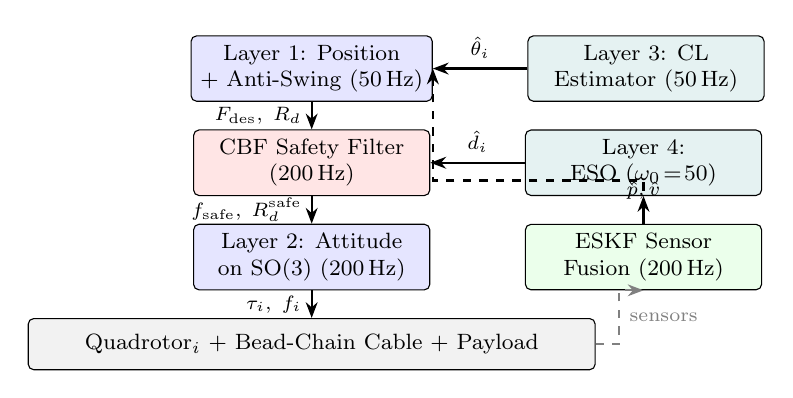
\begin{tikzpicture}[
  block/.style={draw, rounded corners=2pt, minimum width=3.0cm, minimum height=0.65cm, font=\footnotesize, align=center},
  arr/.style={-{Stealth[length=2mm]}, thick},
  every node/.style={font=\footnotesize}
]
  \node[block, fill=blue!10] (L1) {Layer 1: Position\\+ Anti-Swing (50\,Hz)};
  \node[block, fill=red!10, below=0.35cm of L1] (CBF) {CBF Safety Filter\\(200\,Hz)};
  \node[block, fill=blue!10, below=0.35cm of CBF] (L2) {Layer 2: Attitude\\on SO(3) (200\,Hz)};
  \node[block, fill=teal!10, right=1.2cm of L1] (L3) {Layer 3: CL\\Estimator (50\,Hz)};
  \node[block, fill=teal!10, right=1.2cm of CBF] (L4) {Layer 4:\\ESO ($\omega_0\!=\!50$)};
  \node[block, fill=green!8, right=1.2cm of L2] (ESKF) {ESKF Sensor\\Fusion (200\,Hz)};
  \node[block, fill=gray!10, below=0.35cm of L2, minimum width=7.2cm] (plant) {Quadrotor$_i$ + Bead-Chain Cable + Payload};
  \draw[arr] (L1) -- node[left, font=\scriptsize]{$F_{\text{des}},\; R_d$} (CBF);
  \draw[arr] (CBF) -- node[left, font=\scriptsize]{$f_{\text{safe}},\; R_d^{\text{safe}}$} (L2);
  \draw[arr] (L2) -- node[left, font=\scriptsize]{$\tau_i,\; f_i$} (plant);
  \draw[arr] (L3) -- node[above, font=\scriptsize]{$\hat{\theta}_i$} (L1);
  \draw[arr] (L4) -- node[above, font=\scriptsize]{$\hat{d}_i$} (CBF);
  \draw[arr] (ESKF) -- node[above, font=\scriptsize]{$\hat{p},\hat{v}$} (L4);
  \draw[arr, dashed] (ESKF.north) -- ++(0,0.55) -| (L1.east);
  \draw[arr, dashed, gray] (plant.east) -- ++(0.3,0) |- node[right, near start, font=\scriptsize, text=gray]{sensors} (ESKF.south);
\end{tikzpicture}
}
\caption{GPAC per-agent architecture. Blue: control cascade. Red: CBF safety overlay. Teal: estimation. Green: sensor fusion. Each agent executes this pipeline independently; no payload, cable, or estimator states are exchanged (only neighbor GPS positions for collision avoidance).}
\label{fig:architecture}
\end{figure}

\subsection{Layer 1: Position Tracking and Anti-Swing Control}

The outermost layer (${\sim}50$\,Hz) computes a desired thrust vector: $F_{\text{des},i} = F_{\text{fb},i} + F_{\text{ff},i} + F_{\text{cable},i} + F_{\text{swing},i} + F_{\text{eso},i}$, combining five physically motivated components. The PID trajectory tracking feedback (with per-axis anti-windup at $|e_{I,k}| \leq 2.0$) is $F_{\text{fb},i} = -K_p\,e_{p_i} - K_d\,e_{v_i} - K_i\,e_{I_i}$,with $K_p\!=\!\diag(6,6,8)$, $K_d\!=\!\diag(8,8,10)$, $K_i\!=\!\diag(0.1,0.1,0.2)$. The feedforward term compensates gravity and the nominal trajectory: $F_{\text{ff},i} = m_Q(a_{d_i} + ge_3)$.

Cable tension compensation prevents the position controller from treating cable force as a disturbance: $F_{\text{cable},i} = \kappa_T(t)\,T_i\,q_i$, where $\kappa_T(t) = \min\!\bigl(1,\,(t - t_{\text{taut},i})/\Delta_{\text{ramp}}\bigr)$,
and $t_{\text{taut},i}$ is the time cable~$i$ first reaches $T_i \geq 1.0$\,N and $\Delta_{\text{ramp}} = 2$\,s. The gain ramp gradually enables tension compensation using only the \emph{measured} cable force---no knowledge of $m_L$ or $N$ is required. This prevents impulsive loading during the slack-to-taut transition while remaining fully consistent with the decentralized estimation pipeline.

Anti-swing control suppresses pendular oscillations intrinsically on $\Sph^2$, i.e. $F_{\text{swing},i} = k_q\,e_{q_i} - k_\omega\,\omega_{q_i}$,
with $k_q\!=\!4.0$, $k_\omega\!=\!2.0$ ~\cite{lee2018geometric}. Here $e_{q_i}$~\eqref{eq:eq} steers $q_i \to q_{d_i}$ along the geodesic and $\omega_{q_i} \in T_{q_i}\Sph^2$ is the cable angular velocity. Together, these terms reduce $\Psi_{q_i}$ monotonically in the absence of external perturbation. The ESO disturbance estimate (Layer~4) is fed forward as $F_{\text{eso},i} = m_Q\hat{d}_i$.

The desired rotation $R_{d_i} \in \SOthree$ is extracted from $F_{\text{des},i}$ by aligning the body $z$-axis with the thrust direction~\cite{lee2010geometric}:
\begin{equation}
  b_{3c} = \frac{F_{\text{des},i}}{\norm{F_{\text{des},i}}},\;\; b_{2c} = \frac{b_{3c} \times b_{1d}}{\norm{b_{3c} \times b_{1d}}},\;\; b_{1c} = b_{2c} \times b_{3c},
  \label{eq:Rd_extract}
\end{equation}
with $b_{1d} = [\cos\psi_d,\, \sin\psi_d,\, 0]^\top$ setting the desired heading.

\subsection{Layer 2: Geometric Attitude Control on SO(3)}

The inner attitude loop (200\,Hz) applies the geometric tracking controller~\cite{lee2010geometric}:
\begin{equation}
  \tau_i = -k_R\,e_{R_i} - k_\Omega\,e_{\Omega_i} + \Omega_i \times J\Omega_i,
  \label{eq:att_ctrl}
\end{equation}
with $k_R\!=\!8.0$, $k_\Omega\!=\!1.5$, and angular velocity error $e_{\Omega_i} = \Omega_i - R_i^\top R_{d_i}\Omega_{d_i}$. The first two terms provide proportional-derivative control on $\SOthree$; the third compensates gyroscopic coupling. The feedforward terms $\hatmap{\Omega_i}R_i^\top R_{d_i}\Omega_{d_i} - R_i^\top R_{d_i}\dot{\Omega}_{d_i}$ are omitted under the simplification $\Omega_{d_i} \approx 0$ (valid when the desired thrust direction varies slowly relative to the 200\,Hz attitude bandwidth).

\begin{proposition}[Almost-global exponential stability~\cite{lee2010geometric}]\label{prop:lyap}
Define the Lyapunov function
\begin{equation}
  V_R = \tfrac{1}{2}k_R\,\Psi_{R_i} + \tfrac{1}{2}e_{\Omega_i}^\top J\,e_{\Omega_i} + c\,e_{R_i}^\top J\,e_{\Omega_i},
  \label{eq:VR}
\end{equation}
where $\Psi_{R_i} = \frac{1}{2}\tr(I - R_{d_i}^\top R_i)$ is the attitude configuration error and $c>0$ is sufficiently small. Under~\eqref{eq:att_ctrl} with $\Psi_{R_i}(0)<2$:
\begin{equation}
  \dot{V}_R \leq -\lambda_{\min}(W)\bigl(\norm{e_{R_i}}^2 + \norm{e_{\Omega_i}}^2\bigr),
  \label{eq:VR_dot}
\end{equation}
for a positive-definite $W = W(k_R, k_\Omega, J)$, yielding exponential convergence on the dense open set $\{\Psi_R < 2\} \subset \SOthree$.
\end{proposition}

\subsection{Layers 3--4: ESO and Concurrent Learning Estimator}

\textit{Layer~4} is a third-order Extended State Observer (ESO) per translational axis, modeling the dynamics as a double integrator with lumped disturbance $\ddot{p}_k = b_0 u_k + d_k(t)$, $b_0 = 1/m_Q$:
\begin{equation}
  \dot{\hat{z}}_{1k} = \hat{z}_{2k} + 3\omega_0\tilde{x}_k,\;\; \dot{\hat{z}}_{2k} = \hat{z}_{3k} + 3\omega_0^2\tilde{x}_k + b_0 u_k,\;\; \dot{\hat{z}}_{3k} = \omega_0^3\tilde{x}_k,
  \label{eq:eso}
\end{equation}
with $\tilde{x}_k = x_k - \hat{z}_{1k}$ and all poles at $-\omega_0 = -50$\,rad/s (settling time ${\sim}0.1$\,s). The disturbance estimate $\hat{d}_i = [\hat{z}_{3x}, \hat{z}_{3y}, \hat{z}_{3z}]^\top$ is saturated to $|\hat{d}_{i,k}| \leq 20$\,m/s$^2$ and fed forward via $F_{\text{eso},i}$. Under bounded $\dot{d}$, the estimation error scales as $O(\sup|\dot{d}|/\omega_0)$~\cite{guo2013active}.

\textit{Layer~3} adaptively estimates $\hat{\theta}_i \approx m_L/N$ via concurrent learning~\cite{chowdhary2010concurrent}, providing the gravity compensation term $\hat{\theta}_i(ge_3 + \ddot{p}_d^L)$ to Layer~1. The full derivation is given in Section~\ref{sec:estimation}.

\subsection{Cascade Stability and Fault Containment}

The four-layer cascade exploits deliberate timescale separation: attitude ($k_R/J \approx 200$\,rad/s) $\gg$ ESO ($\omega_0 = 50$\,rad/s) $\gg$ position ($K_p/m_Q \approx 5$\,Hz). Standard singular perturbation arguments~\cite{khalil2002nonlinear} guarantee composite stability when this bandwidth ratio exceeds a computable threshold. The hierarchical structure also provides fault containment: mass estimation errors (Layer~3) affect only the feedforward in Layer~1 without corrupting attitude tracking; ESO transients are filtered before reaching the attitude loop; and CBF interventions are bounded by the tilt constraint (Section~\ref{sec:safety}). This modularity supports independent verification of each layer~\cite{koopman2017autonomous}.


\section{Decentralized Adaptive Estimation}\label{sec:estimation}
% !TEX root = ../Main.tex
\begin{figure}[t!]
  \centering
  \includegraphics[width=0.84\columnwidth]{Figures/fig_mass_convergence.png}
  \caption{Adaptive mass estimation convergence. \textit{Top:} Per-quadrotor concurrent learning estimates $\hat{\theta}_i \to m_L/N = 1.0$\,kg, converging within $\sim$8\,s. \textit{Bottom:} Comparison with gradient-only adaptation, which requires $\sim$22\,s and exhibits larger steady-state oscillation.}
  \label{fig:mass_convergence}
\end{figure}

Each quadrotor runs three estimators in a downward cascade---no payload, cable, or adaptive-parameter states are exchanged: (i)~ESKF for navigation, (ii)~geometric load-state filter, and (iii)~concurrent learning mass estimator. Timescale separation---navigation at 200\,Hz versus load/mass estimation at 50\,Hz---lets each layer treat inputs as quasi-static, with upstream errors propagating unidirectionally to simplify stability analysis.

\subsection{Navigation: Error-State Kalman Filter}

A 15-state ESKF~\cite{sola2017quaternion} with $\delta x = [\delta p,\,\delta v,\,\delta\theta,\,\delta b_a,\,\delta b_g]^\top \in \R^{15}$ fuses IMU (200\,Hz), GPS (10\,Hz), and barometer (25\,Hz). Propagation uses bias-corrected specific force $a_W = R(\bar{q})(\tilde{a} - b_a) - ge_3$ and angular velocity $\omega_c = \tilde{\omega} - b_g$. Covariance propagation uses the error-state Jacobian: $P \leftarrow \Phi P\Phi^\top + Q_d$. GPS and barometer corrections use the Joseph-form covariance formula, with the barometer providing altitude observability during GPS outages. The ESKF provides $(\hat{p}_i, \hat{v}_i, \hat{R}_i)$ to all downstream layers; control closes through the estimator, not ground truth.

\subsection{Decentralized Load-State Estimation}

When cable~$i$ is taut, payload position is estimated geometrically: $z_{p_i} = \hat{p}_i - L_i\,n_i$, where $n_i \in \Sph^2$ points from quadrotor to payload and $L_i$ is cable rest length. Each quadrotor maintains a Kalman filter with state $[\hat{p}_{L,i}^\top, \hat{v}_{L,i}^\top]^\top \in \R^6$. The prediction uses a constant-velocity model with damping ($\beta_v = 0.05$), biasing the payload velocity toward the quadrotor velocity, reflecting the quasi-static assumption during slow transport. Measurement noise is modulated by tension confidence:
\begin{equation}
  \xi_T = \min\!\left(1,\,T_i/T_{\text{conf}}\right), \quad R_k \leftarrow R_k / (0.1 + 0.9\,\xi_T),
  \label{eq:tconf}
\end{equation}
with $T_{\text{conf}} = 20$\,N. When the cable is slack, measurement variance inflates and the filter relies on prediction. An outlier gate ($\kappa_\nu = 3.0$) prevents cable whip from corrupting estimates.

With a single cable, payload position is observable only along the cable direction; tangential components depend on prediction. Section~\ref{sec:results} quantifies this gap: the decentralized estimator is roughly $4\times$ worse than a centralized baseline that fuses all $N$ cable constraints but requires inter-agent communication.

From the per-cable vertical force equilibrium of~\eqref{eq:payload}, each quadrotor constructs a scalar parametric model:
\begin{equation}
  \underbrace{T_i \cos\phi_i}_{\varphi_i} = \underbrace{\norm{g\,e_3 + \hat{a}_L}}_{Y_i} \cdot \underbrace{\frac{m_L}{N}}_{\theta} + \varepsilon_i,
  \label{eq:regressor}
\end{equation}
where $\phi_i = \arccos(-n_{i,z})$ is cable angle from vertical, $\hat{a}_L$ is payload acceleration (via numerical differentiation with low-pass filter, $\tau_f = 0.1$\,s), and $\varepsilon_i$ captures modeling error from non-equilibrium dynamics, cable sag, and length asymmetry. Unequal cable lengths cause per-cable vertical force $T_i\cos\phi_i$ to deviate from $m_Lg/N$; this enters $\varepsilon_i$ and increases the ultimately bounded error. In simulation, 19\% cable asymmetry yields steady-state error below 0.1\,kg per agent.

\textit{Implicit coordination.}
The regressor~\eqref{eq:regressor} formalizes the implicit coordination stated in~\eqref{eq:force_convergence}. With feedforward $F_{\text{ff},i} = \hat{\theta}_i \cdot u$ where $u := g\,e_3 + \ddot{p}_L^d$, as $\hat{\theta}_i \to m_L/N$ per agent the total feedforward satisfies
\begin{equation}
  \textstyle\sum_{i=1}^{N} F_{\text{ff},i} = \sum_{i=1}^{N} \hat{\theta}_i\, u \;\longrightarrow\; m_L\, u.
  \label{eq:implicit_coord}
\end{equation}
No agent requires knowledge of $N$ or $m_L$; each estimates its share from local cable measurements, and summation yields correct collective compensation. This holds because the regressor $Y_i$ and control $u$ derive from the same shared trajectory, ensuring scalar parametric consistency across agents.

\begin{remark}[Trajectory synchronization]\label{rem:sync}
Since the trajectory is a polynomial stored locally and evaluated analytically, agents compute $u$ identically up to floating-point precision ($\sim\!10^{-15}$ relative error). Any clock offset $\Delta t$ introduces feedforward error bounded by $\norm{\partial u/\partial t}\Delta t$, which is $O(\Delta t)$\,m/s$^2$ at the tested velocities.
\end{remark}

The concurrent learning update augments gradient descent with stored data is
$\dot{\hat{\theta}}_i = -\gamma\,Y_i\,s_{\text{proj}} - \gamma\rho \sum_{j=1}^{M_i} Y_j(Y_j\hat{\theta}_i - \varphi_j)$, where $\gamma = 0.5$, $\rho = 0.5$, and $s_{\text{proj}} = s_i^\top n_i$ projects sliding variable $s_i = \dot{e}_{L,i} + \lambda e_{L,i}$ ($\lambda = 1.0$) onto cable direction~\cite{chowdhary2010concurrent}. The first term drives online gradient descent; the second replays stored pairs $\{(Y_j, \varphi_j)\}_{j=1}^{M_i}$. The history buffer holds up to $\bar{M} = 50$ points, admitting samples only when excitation exceeds $Y_{\min} = 0.5$\,m/s$^2$ and the regressor differs from the buffer mean by $\delta_Y = 0.1$, ensuring diversity. Estimates are projected to $[\theta_{\min}, \theta_{\max}] = [0.1, 50.0]$\,kg.

\begin{proposition}[Convergence without PE]\label{prop:cl}
If $\Sigma_Y = \frac{1}{M}\sum_j Y_j^2 > 0$ (at least one informative sample), the parameter error satisfies an exponential bound; $\abs{\tilde{\theta}(t)} \leq \abs{\tilde{\theta}(0)}\exp(-\gamma\rho\,\Sigma_Y\,t)$, independently of online excitation. With bounded modeling error $|\varepsilon_i| \leq \bar{\varepsilon}$, convergence is uniformly ultimately bounded: $|\tilde{\theta}| \leq \bar{\varepsilon}/(\rho\,\Sigma_Y)$.
\end{proposition}

\begin{proof}
With $V_\theta = \tilde{\theta}^2/(2\gamma)$, the time derivative has two contributions. The online gradient term contributes $-\tilde{\theta}\,Y_i\,s_{\text{proj}}$; under projection onto $[\theta_{\min}, \theta_{\max}]$, $-\tilde{\theta}\,\text{Proj}(\cdot) \leq 0$~\cite{chowdhary2013exponentially}, so this term only strengthens the bound and its omission is conservative. The concurrent learning term gives $\dot{V}_\theta \leq -\gamma\rho\Sigma_Y\tilde{\theta}^2$; Gr\"{o}nwall's inequality yields exponential bound. Bounded $|\varepsilon_i| \leq \bar{\varepsilon}$ introduces a residual limiting convergence to the UUB ball. The convergence rate $\gamma\rho\Sigma_Y$ depends on trajectory informativeness; empirically, $\sim$30 informative samples accumulated during ascent yield settling in $\sim$8\,s.
\end{proof}


\section{CBF Safety Filter}\label{sec:safety}
% !TEX root = ../Main.tex
A modular CBF layer enforces operational constraints as a minimally invasive post-processing step, modifying the nominal GPAC output only when necessary. Each barrier function corresponds directly to a cooperative transport hazard identified in Section~\ref{sec:intro}, providing runtime supervision within verified safety envelopes.

\subsection{Barrier Function Design}

The safety filter operates on the force vector $f_i \in \R^3$ from Layer~1. Abstracting the translational dynamics~\eqref{eq:quad_trans} as $m_Q\ddot{p}_i = f_i + w_i(t)$ (affine in the control input, with lumped disturbance $w_i$ estimated by the ESO), five barrier functions encode the safe set $\mathcal{C}_k = \{x \mid h_k(x) \geq 0\}$:
\begin{align}
  h_T^{\text{low}} &= T_i - T_{\min},\;\; h_T^{\text{up}} = T_{\max} - T_i & \text{(tautness)}, \label{eq:h_taut}\\
  h_\theta &= \cos\theta_{\max} - \cos\theta_i & \text{(cable angle)}, \label{eq:h_angle}\\
  h_\omega &= \omega_{\max}^2 - \norm{\omega_{q_i}}^2 & \text{(swing rate)}, \label{eq:h_swing}\\
  h_{\text{tilt}} &= \cos\phi_{\max} - \cos\phi_i & \text{(vehicle tilt)}, \label{eq:h_tilt}\\
  h_{\text{col}} &= \norm{p_i - p_j}^2 - d_{\min}^2 & \text{(collision)}, \label{eq:h_col}
\end{align}
with $T_{\min}\!=\!2$\,N, $T_{\max}\!=\!60$\,N, $\theta_{\max}\!=\!0.6$\,rad ($34.4^\circ$), $\omega_{\max}\!=\!1.5$\,rad/s, $\phi_{\max}\!=\!0.5$\,rad ($28.6^\circ$), $d_{\min}\!=\!0.8$\,m. For the collision barrier~\eqref{eq:h_col}, the second derivative involves both $f_i$ and $f_j$; in the decentralized setting, agent~$i$ treats the neighbor's acceleration as a bounded disturbance and enforces a conservative one-sided HOCBF constraint using only its own force input, with the disturbance absorbed into the ISSf margin.

The tautness barriers~\eqref{eq:h_taut} are relative-degree-one. Cable angle, tilt, and collision are relative-degree-two and use HOCBFs~\cite{xiao2022control, ames2019control}: defining $\psi_1 = \dot{h} + \alpha_1 h$, the constraint $\dot{\psi}_1 + \alpha_2\psi_1 \geq 0$ becomes relative-degree-one in the control, with the safe set $\{\psi_1 \geq 0\} \cap \{h \geq 0\}$ rendered forward-invariant.

\subsection{Safety QP with ISSf Guarantees}

The safety filter solves, at each control cycle:
\begin{equation}
  f_{\text{safe}} = \argmin_{f,\,\delta}\;\norm{f - f_{\text{nom}}}^2 + \lambda\!\sum_j\!\delta_j^2 \;\;\text{s.t.}\;\; \dot{h}_j + \alpha_j h_j \geq -\mu_j - \delta_j,
  \label{eq:cbf_qp}
\end{equation}
with $\lambda = 100$ penalizing relaxation. In the presence of disturbances, hard forward invariance of $\{h \geq 0\}$ is unrealistic. We employ the Input-to-State Safety (ISSf) framework, coupling the robustness margin to the ESO estimate:
\begin{equation}
  \dot{h}_j + \alpha_j h_j \geq -\mu_{\text{base}} - \kappa_d\norm{\hat{d}_i},
  \label{eq:issf}
\end{equation}
with $\mu_{\text{base}} = 2.0$, $\kappa_d = 1.5$. When the ESO reports large disturbances, the margin grows and the filter activates earlier. The steady-state violation bound is:
\begin{equation}
  h_j(t) \geq -(\mu_{\text{base}} + \kappa_d\bar{d})/\alpha_j.
  \label{eq:issf_bound}
\end{equation}

\begin{figure}[t]
  \centering
  \includegraphics[width=\columnwidth]{Figures/fig_cbf_activation.png}
  \caption{CBF activation timeline. \textit{Top:} Tension margin (distance to $T_{\min}$) for all cables. \textit{Middle:} Cable angle margin (distance to $\theta_{\max} = 34.4^\circ$); shaded regions indicate CBF activation during aggressive cornering (1.7\% of time). \textit{Bottom:} Tilt margin (never violated). Orange regions denote constraint activation.}
  \label{fig:cbf_activation}
\end{figure}

The tautness constraint requires $\dot{T}_i$, estimated via a second-order Butterworth low-pass ($f_c = 15$\,Hz, $-40$\,dB/dec) applied to finite-difference tension rate, attenuating cable vibrations (${\sim}55$\,Hz) by ${\sim}22$\,dB with ${\sim}11$\,ms group delay.

The implementation uses sequential gradient projection with priority ordering (tautness $>$ angle $>$ tilt $>$ swing $>$ collision) rather than a full QP solver. This approximation is equivalent to~\eqref{eq:cbf_qp} when at most one constraint is active---the typical case, as the CBF is active only 1.7--3.2\% of total simulation time. Consequently, the ISSf guarantees of~\eqref{eq:issf_bound} hold during single-constraint activation. When multiple constraints activate simultaneously (rare; concentrated in $<$0.3\% of time during the sharpest cornering), the sequential method enforces the explicit priority ordering above, producing a feasible but potentially suboptimal solution; the slack variables $\delta_j$ ensure that lower-priority constraints degrade gracefully. The per-agent cost is $O(N_c)$ with $N_c = 6$ constraints (${\sim}1200$\,FLOPs/cycle).

\subsection{Compatibility with Geometric Attitude Control}

The safety filter modifies the force direction, which changes the desired rotation $R_d$. A critical requirement is that this perturbation does not exit the almost-global stability region of the geometric controller.

\begin{theorem}[Safety-Stability Compatibility]\label{thm:compatibility}
Suppose the tilt barrier~\eqref{eq:h_tilt} with $\phi_{\max}=0.5$\,rad is enforced. Then the attitude error between the nominal and safe desired rotations satisfies:
\begin{equation}
  \Psi_R(R_d^{\text{nom}}, R_d^{\text{safe}}) \leq 1 - \cos(2\phi_{\max}) \approx 0.46 < 1,
  \label{eq:compat}
\end{equation}
and the geometric attitude controller retains almost-global exponential stability.
\end{theorem}

\begin{figure}[t]
  \centering
  \includegraphics[width=\columnwidth]{Figures/fig_safety_constraints.png}
  \caption{Safety constraint satisfaction. \textit{Top:} Cable angle from vertical for each cable, with the CBF limit $\theta_{\max} = 34.4^\circ$ (dashed). Brief excursions above the limit during aggressive cornering remain within the ISSf margin. \textit{Bottom:} Quadrotor tilt angle with limit $\phi_{\max} = 28.6^\circ$ (dashed); the constraint is never violated.}
  \label{fig:safety_constraints}
\end{figure}

\begin{proof}
The tilt constraint bounds $\phi_i \leq \phi_{\max}$, so the angle between $f_{\text{nom}}$ and $f_{\text{safe}}$ satisfies $\vartheta \leq 2\phi_{\max} = 1.0$\,rad. Since $R_d$ aligns $b_{3c} = f/\norm{f}$~\eqref{eq:Rd_extract}, a rotation by $\vartheta$ gives $\Psi_R(R_d^{\text{nom}}, R_d^{\text{safe}}) = 1 - \cos\vartheta \leq 0.46$. As $\Psi_R(R_i, R_d^{\text{nom}}) \to 0$ exponentially (Proposition~\ref{prop:lyap}), subadditivity of $\Psi_R$~\cite{lee2010geometric} yields $\Psi_R(R_i, R_d^{\text{safe}}) < \varepsilon + 0.46 < 2$ after settling (${\sim}0.1$\,s).
\end{proof}

\begin{remark}[Timescale separation]\label{rem:timescale}
The compatibility result relies on three well-separated timescales: the \emph{fast} attitude loop ($k_R/J \approx 200$\,rad/s, settling ${\sim}5$\,ms), the \emph{medium} safety filter (Butterworth cutoff $2\pi \times 15 \approx 94$\,rad/s), and the \emph{slow} position/cable dynamics ($\sqrt{g/L} \approx 3$\,rad/s). Since the fast dynamics settle (${\sim}5$\,ms) an order of magnitude faster than force modifications evolve (${\sim}50$--$200$\,ms), standard singular perturbation analysis~\cite{khalil2002nonlinear} ensures the attitude controller tracks the slowly varying $R_d^{\text{safe}}$ without losing stability. This bandwidth hierarchy $\omega_{\text{att}} \gg \omega_{\text{CBF}} \gg \omega_{\text{pos}}$ is the structural condition making the layered architecture composable.
\end{remark}


\section{Simulation Results}\label{sec:results}
% !TEX root = ../Main.tex
We validated GPAC using a Drake-based~\cite{drake2024} multibody simulation, with parameters listed in Table~\ref{tab:params}. The physics engine runs at 5000 Hz using a semi-implicit Euler method, and cable vibrations (around 55 Hz) are resolved with 90 times oversampling. The cable rest lengths are asymmetric ([0.914, 1.105, 0.995] m), showing up to 19\% variation. The multi-rate timing is set to match the GPAC layer structure. The simulation environment includes Dryden wind and a full sensor suite. All control loops are closed using the ESKF rather than ground truth, ensuring sensor-in-the-loop realism.

The overall 3D RMSE is 22.9 cm, which is 3.3\% of the workspace diagonal and well within one cable length. This result is achieved without centralized coordination, even with wind disturbance and 19\% cable asymmetry. A 15-seed Monte Carlo test confirms the results are representative (6.3\% CV). Most of the error is horizontal because pendulum dynamics amplify lateral disturbances, while vertical error is well controlled through direct thrust-altitude coupling and barometer-aided estimation. The largest errors occur during figure-eight cornering, but performance improves as concurrent learning collects more data.

\begin{figure}[t]
  \centering
  \includegraphics[width=0.84\columnwidth]{Figures/fig_trajectory_3d.png}
  \caption{3D trajectory of the load and the quadcopters. The max velocity of the load is 1\,m/s.}
  \label{fig:trajectory_3d}
\end{figure}

\begin{table}[t]
  \centering
  \caption{Payload tracking errors (cm).}
  \label{tab:tracking}
  \begin{tabular}{@{}lcccccc@{}}
    \toprule
    & \multicolumn{2}{c}{\textbf{Horiz.}} & \multicolumn{2}{c}{\textbf{Vert.}} & \multicolumn{2}{c}{\textbf{3D}} \\
    \textbf{Phase} & RMSE & Max & RMSE & Max & RMSE & Max \\
    \midrule
    Ascent (2--6\,s) & 8.9 & 26.7 & 11.0 & 25.9 & 14.2 & 28.3 \\
    Fig-8 right (7--20\,s) & 26.6 & 79.9 & 4.0 & 10.7 & 26.9 & 80.3 \\
    Fig-8 left (24--36\,s) & 17.6 & 37.5 & 3.6 & 9.4 & 18.0 & 37.7 \\
    Descent (39--43\,s) & 13.1 & 27.1 & 9.0 & 16.4 & 16.0 & 27.3 \\
    Post-descent (43--50\,s) & 7.7 & 12.4 & 1.6 & 4.8 & 7.9 & 12.5 \\
    \midrule
    \textbf{Overall} & 22.2 & 79.9 & 5.4 & 25.9 & \textbf{22.9} & 80.3 \\
    \bottomrule
  \end{tabular}
\end{table}

\begin{figure}[t]
  \centering
  \includegraphics[width=0.84\columnwidth]{Figures/fig_tracking_error.png}
  \caption{Payload tracking error. \textit{Top:} 3D error (RMSE 22.9\,cm); peaks (80.3\,cm) during aggressive cornering. \textit{Bottom:} Components. The right loop (7--20\,s) shows larger errors before CL converges.}
  \label{fig:tracking_error}
  \vspace{-5pt}
\end{figure}

\begin{figure}[t]
  \centering
  \includegraphics[width=0.84\columnwidth]{Figures/fig_estimation_error.png}
  \caption{Estimation performance. \textit{Top:} ESKF error (7.1\,cm RMSE, max 22.3\,cm during cornering). \textit{Middle:} Decentralized load estimate (49.5\,cm RMSE), limited by single-cable observability. \textit{Bottom:} Per-quadrotor mass estimates converging to $m_L/N$.}
  \label{fig:estimation_error}
  \vspace{-5pt}
\end{figure}

Table~\ref{tab:tracking} shows payload tracking errors for the baseline seed. The overall 3D RMSE is 22.9 cm, which is 3.3\% of the workspace diagonal and well within one cable length. This result is achieved without centralized coordination, even with wind disturbance and 19\% cable asymmetry. A 15-seed Monte Carlo test confirms the results are representative (6.3\% CV). Most of the error is horizontal because pendulum dynamics amplify lateral disturbances, while vertical error remains low thanks to direct thrust-altitude control and barometer-aided estimation. The largest errors occur during figure-eight cornering, but performance improves as concurrent learning collects more data.

The ESKF gives quadrotor position RMSE that matches the GPS noise floor, though errors increase during cornering. Low variance across Monte Carlo seeds shows that ESKF accuracy depends on sensor noise, not cable geometry. The decentralized load estimator has a 49.5 cm RMSE, which is 4 times worse than the centralized oracle's 12.4 cm RMSE. This difference is due to the single-cable observability limit discussed in Section~\ref{sec:estimation}. The centralized baseline needs about 29 kbps of bandwidth.

Concurrent learning converges in about 8 seconds, collecting around 30 useful samples during ascent. Without concurrent learning ($\rho = 0$), settling takes much longer and oscillations are larger (see Table~\ref{tab:failure_modes}).

Table~\ref{tab:failure_modes} shows the hazard-to-mitigation mapping and constraint enforcement data. The cable angle CBF is activated most often; the observed excursion (48.1° compared to the 34.4° limit) and swing rate (1.6 vs. 1.5 rad/s) match the ISSf bound, which predicts margin violations of this size during peak disturbance. Tilt and collision constraints are never violated (clearance is at least 1.04 m, which is 30\% above $d_{\min}$). The CBF is rarely activated and only increases tracking RMSE by 2\%.

Table~\ref{tab:ablation} breaks down each component's impact. The ESO provides the greatest benefit, as removing it results in a 43\% drop in performance. Concurrent learning is next, with a 33\% decrease. This order shows that handling wind disturbance is the main factor affecting tracking accuracy here, which aligns with the Dryden turbulence intensities used. The CBF has little effect on tracking cost but greatly reduces peak cable angles. The centralized estimation baseline lowers RMSE by 22\%, but it requires agents to communicate.

\begin{table}[t]
  \centering
  \caption{Ablation results: payload tracking RMSE (cm).}
  \label{tab:ablation}
  \begin{tabular}{@{}lccc@{}}
    \toprule
    \textbf{Configuration} & \textbf{RMSE} & $\boldsymbol{\Delta}$ & \textbf{Max Angle} \\
    \midrule
    Full GPAC (baseline) & 22.9 & --- & 48.1$^\circ$ \\
    No concurrent learning & 31.7 & +33\% & 42.1$^\circ$ \\
    No ESO feedforward & 34.1 & +43\% & 44.8$^\circ$ \\
    No CBF safety filter & 24.2 & +2\% & 52.0$^\circ$ \\
    Centralized estimation & 18.5 & $-$22\% & 38.2$^\circ$ \\
    \bottomrule
  \end{tabular}
\end{table}

\begin{table}[t]
  \centering
  \caption{Cable tension statistics (N) during steady-state flight. Asymmetric cable lengths produce unequal load sharing.}
  \label{tab:tension_stats}
  \begin{tabular}{@{}lccccc@{}}
    \toprule
    \textbf{Cable} & $\boldsymbol{L_i}$ \textbf{(m)} & \textbf{Mean} & \textbf{Std} & \textbf{Min} & \textbf{Max} \\
    \midrule
    0 & 0.914 & 14.88 & 3.31 & 1.52 & 26.34 \\
    1 & 1.105 & 10.23 & 3.14 & 2.00 & 22.16 \\
    2 & 0.995 & 13.03 & 2.75 & 6.07 & 19.96 \\
    \bottomrule
  \end{tabular}
\end{table}

\begin{figure}[t]
  \centering
  \includegraphics[width=0.84\columnwidth]{Figures/fig_cable_tensions.png}
  \caption{Cable tensions. Asymmetric lengths yield unequal load sharing accommodated without coordination.}
  \label{fig:cable_tensions}
  \vspace{-5pt}
\end{figure}

\begin{table}[t]
  \centering
  \caption{Hazard-to-mitigation mapping with constraint limits and measured performance.}
  \label{tab:failure_modes}
  \begin{tabular}{@{}llccc@{}}
    \toprule
    \textbf{Hazard} & \textbf{Mitigation} & \textbf{Limit} & \textbf{Observed}\\
    \midrule
    Mass unknown & CL estimation & --- & $\hat{\theta} \!\to\! m_L/N$, 8\,s\\
    Wind disturbance & ESO feedfwd & --- & +43\% w/o\\
    Cable slack & CBF tension & {[2, 60]\,N} & {[1.5, 26.3]\,N}\\
    Cable angle & CBF + anti-swing & $34.4^\circ$ & $48.1^\circ$\\
    Excessive tilt & CBF tilt & $28.6^\circ$ & $25.1^\circ$\\
    Swing rate & CBF swing & 1.5\,rad/s & 1.6\,rad/s\\
    Collision & CBF separation & 0.8\,m & $\geq 1.04$\,m\\
    Sensor noise & ESKF fusion & --- & 6.9\,cm RMSE\\
    \bottomrule
  \end{tabular}
\end{table}


\section{Conclusion}\label{sec:conclusion}

This paper presented GPAC, a four-layer hierarchical controller for decentralized cooperative aerial transport on $\SEthree \times (\Sph^2)^N$. Each quadrotor runs an identical control and estimation stack using only local sensors and its cable attachment---no knowledge of $N$ or $m_L$ is required, and no payload, cable, or adaptive-parameter states are exchanged (only neighbor GPS positions for collision avoidance). Concurrent learning enables mass estimation without persistent excitation (converging in ${\sim}8$\,s, +33\% over gradient-only), and a modular CBF safety filter enforces operational constraints with ISSf guarantees provably compatible with the geometric attitude controller (Theorem~\ref{thm:compatibility}). High-fidelity Drake simulation with flexible bead-chain cables, ESKF sensor fusion, and Dryden wind validates 22.9\,cm tracking RMSE at under 1\,MFLOP/s per agent.

The hazard-oriented architecture---where each layer directly mitigates a specific transport risk (Table~\ref{tab:failure_modes})---combines formal stability certificates, adaptive learning, and runtime constraint enforcement without centralized coordination. The hierarchical timescale separation limits fault propagation, the decentralized implementation eliminates single points of failure, and the per-agent policy is invariant to team size by construction. These properties position GPAC toward assurance-oriented deployment of multi-UAV transport systems.

\textit{Limitations.} All results are simulation-only; hardware validation is the immediate next step. The shared broadcast trajectory is a single point of failure. The decentralized load estimator exhibits a $4\times$ gap versus the centralized baseline (49.5 vs.\ 12.4\,cm), motivating distributed consensus-based estimation. Agent dropout and dynamic reconfiguration are not addressed. The sequential CBF projection can be suboptimal when multiple constraints activate simultaneously.

\textit{Future work.} Flight experiments with 3--6 quadrotors, distributed estimation to narrow the centralized gap while preserving communication efficiency, agent dropout detection and $N$-adaptive mass re-estimation, and full QP-based multi-constraint resolution for the safety filter.


% ======================== REFERENCES ============================
\bibliographystyle{IEEEtran}
\bibliography{References/References}

\end{document}
